\documentclass[11pt,a4paper,oneside,numbers=noenddot,bibliography=totoc]{scrreprt}
\pdfminorversion=7 % the Graphviz-generated figure PDFs are version 1.7

\usepackage[T1]{fontenc}
\usepackage{lmodern}
\usepackage[english]{babel}
\usepackage[a4paper,top=2.3cm,bottom=2.3cm,left=2.4cm,right=2.4cm]{geometry}
\usepackage{microtype}
\usepackage{csquotes}
\usepackage{booktabs}
\usepackage{array}
\usepackage{siunitx}
\usepackage{graphicx}
\graphicspath{{figures/}}
\usepackage{amsmath}
\usepackage[style=ieee,backend=biber,urldate=iso,seconds=true]{biblatex}
\usepackage[hidelinks]{hyperref}
\usepackage[capitalise,noabbrev]{cleveref}
\usepackage{etoolbox}

% Chapters flow continuously instead of each starting a new page, but keep a
% clear gap before every chapter title. KOMA issues the chapter page break in
% \scr@startchapter; gate it behind \if@chapflow so front/back matter (title,
% declaration, abstract, bibliography, appendix) still break, while body
% chapters flow. \if@chapflow is toggled on/off in the document body.
\newif\ifchapflow \chapflowfalse
\makeatletter
\patchcmd{\scr@startchapter}
  {\if@openright\cleardoublepage\else\clearpage\fi}
  {\ifchapflow\else\if@openright\cleardoublepage\else\clearpage\fi\fi}
  {}{\typeout{PATCHFAIL: scr@startchapter chapter-break gate}}
\makeatother
\RedeclareSectionCommand[beforeskip=-\baselineskip,afterskip=.7\baselineskip]{chapter}
\renewcommand*{\chapterheadstartvskip}{\vspace{3\baselineskip}}

\addbibresource{refs.bib}

\sisetup{
  round-mode = places,
  round-precision = 3,
  table-format = 1.3,
}

\title{Relational Alpha Factors with Graph Attention Networks:\\
A Dual-Track Study on US Equities and European Power Markets}
\author{Wentao Ma}
\date{July 8, 2026}

\begin{document}

\begin{titlepage}
  \centering

  \vspace*{2em}
  {\large Westphalian University of Applied Sciences, Gelsenkirchen\par}
  \vspace{0.35em}
  {\normalsize Department of Computer Science and Communication\par}

  \vspace{3.2em}
  {\scshape\large Wissenschaftliche Vertiefung Informatik\par}
  \vspace{0.3em}
  {\normalsize Scientific Capstone Project --- Technical Report\par}

  \vspace{5em}
  {\sffamily\bfseries\huge Relational Alpha Factors with\\[0.4em]
  Graph Attention Networks\par}
  \vspace{1.2em}
  {\sffamily\large A Dual-Track Study on US Equities and\\[0.2em]
  European Power Markets\par}

  \vspace{5em}
  {\Large\bfseries Wentao Ma\par}
  \vspace{0.4em}
  {\normalsize\texttt{ma.wentao@studmail.w-hs.de}\par}
  \vspace{0.25em}
  {\normalsize M.Sc.\ Informatik\par}

  \vfill

  {\normalsize
  \begin{tabular}{@{}rl@{}}
    Supervisor: & Prof.\ Laura Anderle\\[0.25em]
    Module:     & Wissenschaftliche Vertiefung Informatik, 12\,ECTS\\[0.25em]
    Submitted:  & Gelsenkirchen, July 8, 2026\\
  \end{tabular}\par}

  \vspace{1.5em}
\end{titlepage}

\chapter*{Declaration of Originality}

I hereby declare that I have written this report independently and without
outside assistance, and that I have used no sources or aids other than those
cited. All passages taken verbatim or in substance from published or
unpublished work of others are identified as such. This report has not been
submitted, in the same or a similar form, to any other examination authority.

\vspace{3em}
\noindent Gelsenkirchen, July 8, 2026\hfill Wentao Ma

\chapter*{Abstract}

Cross-sectional alpha factors score assets in isolation, yet the assets
are coupled --- statistically in equity markets, physically in European
power markets. This report measures what that coupling structure is
worth. To make the measurement interpretable, the information set is
held fixed and two questions are separated: what a graph adds, measured
against an unlearned uniform-propagation anchor, and what learned
attention adds, measured as a graph attention network's margin over that
anchor on the same topology. One GAT kernel, one leakage-controlled
evaluation harness, and one suite of research gates run on two
structurally different graphs: an estimated correlation backbone over 49
US equities and the physical interconnector network over 20 European
bidding zones.

On equities, learned attention beats unlearned propagation in 30 of 30
seeded runs; the best configuration reaches an out-of-sample rank-IC of
$0.0148 \pm 0.0043$ and long-short Sharpe of $1.37 \pm 0.39$ over five
seeds. The resulting composite factor is unique, consistent, and robust
--- three of four gates --- but never beats the best single input
factor. Attention analysis explains the modesty: the model applies a
stationary, near-uniform reweighting of neighbour pooling, not sharp
selection. On energy, the alpha framing failed in an instructive way:
three nested evaluation artifacts --- overlapping labels, wrong
annualisation, and a clip on the evaluation return that concealed
short-leg tail losses --- each produced spectacular numbers before
being caught by the project's own controls, and under honest returns
the strategy loses money. Reframed as forecasting, the energy track
yields the cleanest relational evidence: the interconnector graph lifts
node-level price forecast skill by $+0.131$ over an identically
informed no-graph baseline, and on cross-border spreads --- a target
that does not exist without the relation --- message passing beats a
both-endpoint baseline in five of five seeds ($+0.056$ skill).

The report's contributions are the isolation methodology, the two
measured results, a worked three-artifact cautionary example for
GNN-based market research, and the platform engineering that makes all
of it reproducible from archived artifacts.


\tableofcontents
\clearpage
\chapflowtrue

\chapter{Introduction}
\label{ch:intro}

Quantitative alpha research scores assets one at a time. A formulaic
alpha reads a single stock's prices and volumes and emits a number; the
cross-section of those numbers, ranked, is the signal
\cite{kakushadze2016alphas}. Yet the assets themselves are anything but
isolated: equities co-move within sectors and supply chains, and
European power prices are literally wired together by cross-border
transmission lines. The premise of this project is that the coupling
structure is information, and its subject is a careful measurement of
how much.

The measurement question splits in two, and the split matters. That a
graph-augmented model outperforms a non-relational baseline is easy to
show and hard to interpret --- the gain may come from the graph, from
the extra parameters, or from information the baseline never saw. This
project therefore fixes the information set (the same island alphas
every model consumes) and separates two claims: what the \emph{graph}
adds, measured by an unlearned uniform-propagation anchor, and what
\emph{learned attention} adds, measured as the gap between a graph
attention network \cite{velickovic2018gat} and that anchor on the same
topology. Three research questions organise the work:

\begin{itemize}
  \item[RQ1] Does learned attention add value over unlearned relational
    propagation, holding inputs and topology fixed?
  \item[RQ2] Does one GAT kernel and one evaluation harness transfer
    across structurally different graphs --- an estimated correlation
    backbone over US equities and a physical interconnector network over
    European bidding zones --- without manufacturing false positives?
  \item[RQ3] On real power-market data, does the physical topology
    improve forecast skill, and where does its value concentrate?
\end{itemize}

A reader from outside quantitative finance should carry one picture
through what follows (\cref{sec:bg-primer} defines the recurring
vocabulary). Every model in this report is trained on the same task:
score today's cross-section of assets so that the scores rank the next
period's price moves, five trading days ahead for equities, one day
ahead for power. Every model in a comparison also receives the same
per-asset inputs: ten signals computed from each stock's own prices and
volumes on the equity track, and each zone's price dynamics plus its
published fundamentals (load, wind and solar forecasts among them) on
the energy track. In particular, the graph neural networks here are not
a vehicle for feeding extra data into price prediction --- whatever
exogenous drivers exist go to the graph-free baselines too. The
relational models' only privilege is topological: permission to
exchange information along edges, estimated return correlations for
equities and the physical cross-border grid for power. Every headline
number in this report is therefore a margin, the value of that
permission with everything else held fixed.

The answers, in brief. On the equity track, learned attention beats the
uniform anchor in thirty of thirty seeded runs, and the best
configuration reaches an out-of-sample (OOS) IC of $0.0148 \pm 0.0043$ and
Sharpe of $1.37 \pm 0.39$ over five seeds; the resulting composite
passes three of four research gates but never beats the single best
island alpha, a failure this report states as plainly as the successes
(\cref{ch:equity}). On the energy track the alpha framing collapsed
honestly: three nested evaluation artifacts each produced spectacular
numbers before the project's own controls caught them, and under honest
returns the strategy loses money (\cref{ch:energy}). Reframed as
forecasting, the same track produced the project's cleanest positives:
the interconnector graph lifts node-level price forecast skill by
$+0.131$ over a no-graph baseline with identical drivers, and on the
irreducibly relational target --- cross-border spreads --- message
passing beats a both-endpoint baseline in five of five seeds
(\cref{sec:en-edge}).

Five contributions follow from this, each defended in a named part of
the report. First, an isolation methodology for relational factors:
matched no-learning anchors, four research gates, and structural
leakage controls, defined once in \cref{ch:methodology} and reused
unchanged by every experiment. Second, the equity result itself ---
attention's margin over naive propagation as a distribution over seeds,
devices, and configurations rather than a point estimate, together with
an interpretability analysis showing the mechanism to be a gentle,
stationary reweighting of mean pooling (\cref{ch:equity}). Third, a
worked cautionary example: the energy alpha arc of
\cref{ch:energy}, in which the project's own controls catch three
artifacts in sequence, ending in a verdict --- rank correlation can be
positive while the strategy loses money --- that generalises beyond
power markets. Fourth, the forecasting reframe and its control-validated
graph value, concentrated on the relational target
(\cref{sec:en-forecast,sec:en-edge}). Fifth, the platform engineering
that makes the rest reproducible: two seams that let island and
relational factors share one pipeline, warehouse marts built from
research runs, and a test suite that pins the leakage-critical logic
(\cref{ch:platform}).

A note on standards. This is a Master's capstone report, and the working
assumption throughout is that its most valuable output is not a
headline Sharpe but a defensible measurement process. Wherever a result
died under scrutiny, the scrutiny and the death are in the text; the
negative results are load-bearing, not confessional.

The report proceeds as follows. \Cref{ch:background} places the work in
the alpha-research, GNN, and electricity-forecasting literatures.
\Cref{ch:platform} describes the platform and the two seams.
\Cref{ch:methodology} fixes the measurement apparatus.
\Cref{ch:equity,ch:energy} report the two tracks.
\Cref{ch:discussion} confronts threats to validity, and
\cref{ch:conclusion} closes with what a successor project should do
differently.

\chapter{Background and Related Work}
\label{ch:background}

\section{Alpha research in plain terms}
\label{sec:bg-primer}

This report uses a small vocabulary that is standard in quantitative
finance and opaque outside it; this section defines it once, so that
the rest of the report does not presuppose a finance background.

An \emph{alpha factor} is a rule that assigns every asset a score at
every point in time, constructed so that higher-scored assets should
subsequently outperform lower-scored ones. The prediction is about
\emph{relative} performance within a fixed universe, not about price
levels: the object of interest is the \emph{cross-section} --- all
assets observed at one timestamp --- and whether today's ranking of
scores anticipates the ranking of returns realised over the following
days. A factor that scores an asset from that asset's own history
alone (five-day price reversal, abnormal trading volume) is an
\emph{island factor} in this report's terminology; a \emph{relational
factor} may also read the asset's neighbours in a graph.

Two measurements recur on every page of \cref{ch:equity,ch:energy}.
The \emph{information coefficient} (IC) is the correlation between the
scores issued at a timestamp and the returns realised afterwards; this
report uses the rank form (\emph{rank-IC}, a Spearman correlation),
computed cross-sectionally at each timestamp and averaged. A rank-IC
of 1 would be a perfect ordering; 0 is no predictive skill at all.
Real factors are weak --- the best out-of-sample composite in this
report reaches a rank-IC of about 0.015 (\cref{ch:equity}) --- and
factors of this strength are useful only in combination, which is why
the field builds them in large numbers. The \emph{Sharpe ratio}
evaluates a factor as a trading strategy instead: buy the top-ranked
assets, sell short the bottom-ranked ones (a \emph{long-short}
portfolio, whose exposure to the overall market direction largely
cancels), and divide the strategy's mean return by its volatility,
annualised. The two numbers can disagree, because ranking well says
nothing about the magnitudes of wins and losses; \cref{ch:energy}
turns exactly this disagreement into one of the report's main
findings.

``Alpha'' itself, in the industry idiom this report inherits from
Kakushadze's catalogue of practitioner formulas
\cite{kakushadze2016alphas}, names nothing deeper than a signal
expected to carry predictive information beyond passive market
exposure. No claim below depends on a stricter definition.

\section{Cross-sectional alpha research}
\label{sec:bg-alpha}

The equity track's island factors follow the formulaic-alpha idiom that
Kakushadze documented from industry practice: short arithmetic
expressions over price and volume, evaluated per stock and ranked across
the cross-section each day \cite{kakushadze2016alphas}. Individually
weak and mutually correlated, such alphas are meant to be combined, and
the interesting research questions live in the combination step. Machine
learning has a measured track record here: Gu, Kelly and Xiu showed on
six decades of US data that flexible models --- trees and shallow
networks in particular --- roughly double the predictive $R^2$ of linear
benchmarks for cross-sectional returns, driven largely by interaction
effects that linear factor models cannot express
\cite{gu2020empirical}. The same literature is emphatic about how easily
such gains evaporate under sloppy evaluation. L\'opez de Prado catalogues
the failure modes --- label overlap, missing embargoes, selection on
test data, backtest overfitting --- and the purged, embargoed validation
splits he advocates \cite{lopezdeprado2018afml} are the direct ancestors
of the split protocol in \cref{sec:splits}. This report treats that
methodological literature as load-bearing: two of the energy track's
three artifacts (\cref{sec:en-artifact}) are textbook instances of
exactly the pathologies it names.

\section{Graph neural networks and attention}
\label{sec:bg-gnn}

Graph neural networks compute node representations by aggregating
information from graph neighbourhoods. In the graph convolutional
network of Kipf and Welling, the aggregation weights are fixed by the
graph's degree structure \cite{kipf2017gcn}; graph attention networks
replace them with weights computed from the node features themselves, so
the model learns which neighbours matter for each node
\cite{velickovic2018gat}. Brody, Alon and Yahav later showed that the
original formulation computes a restricted, effectively static form of
attention and proposed GATv2, which reorders the operations to make the
attention genuinely conditional on the query node
\cite{brody2022gatv2}. Both operators are available off the shelf in
PyTorch Geometric \cite{fey2019pyg}; the alpha track uses the original
operator, the forecasting work the GATv2 variant
(\cref{sec:training}).

Applying relational models to stock prediction is an established idea.
Feng et al.\ combine a temporal encoder with relational graphs over
company links and learn to rank stocks by return
\cite{feng2019stockranking}, and much subsequent work follows the same
pattern: propose an architecture, report that it beats non-relational
baselines. This project asks a deliberately narrower question. Rather
than demonstrating that some graph-augmented architecture outperforms,
it holds the information set fixed --- the same island alphas every
baseline consumes --- and measures the marginal value of each
ingredient separately: the graph via an unlearned uniform-propagation
anchor, and learned attention via the gap between the GAT and that
anchor (\cref{sec:anchors}). The price of the narrower question is
weaker headline numbers; the payoff is that when the equity track
reports a positive attention margin in thirty of thirty runs
(\cref{ch:equity}), the claim isolates a mechanism rather than a
model.

\section{Electricity price forecasting}
\label{sec:bg-epf}

Day-ahead electricity prices are set in a daily auction and driven by
fundamentals --- load, wind and solar in-feed, fuel prices --- with
properties equity researchers rarely face: strong diurnal seasonality,
negative prices, and fat-tailed scarcity spikes. Weron's review maps the
field's method families and stresses the role of these fundamentals and
of rigorous out-of-sample evaluation \cite{weron2014epf}; Lago et al.\
sharpen the evaluation point for the deep-learning era, offering an
open benchmark and best practices --- among them, always comparing
against naive and well-tuned simple baselines --- precisely because the
literature is rich in models that beat only weak straw men
\cite{lago2021epf}. The forecast-skill ladder of \cref{sec:skill}, with
persistence pinned at zero skill and a ridge on fundamentals as the
serious no-graph baseline, is this project's implementation of that
advice. Its energy-specific contribution is not a new forecasting
architecture but a controlled measurement of one factor the standard
benchmarks do not isolate: whether the physical interconnector topology
itself adds forecast skill, at the node level and --- where the answer
turns out to be strongest --- for cross-border spreads
(\cref{sec:en-edge}).

\section{Where this report sits}
\label{sec:bg-position}

Against this background, three commitments distinguish this report from
the related work above, which rarely combines them. Every relational
claim is measured against matched no-learning anchors on identical
inputs, so a positive result isolates an ingredient rather than
crediting a whole architecture. One GAT kernel and one evaluation
harness are carried across two structurally different graphs --- an
estimated correlation backbone over equities and a physical transmission
network over bidding zones --- with the negative controls travelling to
both. And the honesty standard of the methodological literature is
applied without exception: negative results (a failed value-added gate,
a money-losing energy strategy, a null congestion hypothesis) are
reported as findings, because the diagnostic arc that produced them is
the part of this work most likely to help a reader.

\chapter{Platform Architecture}
\label{ch:platform}

The research of \cref{ch:equity,ch:energy} runs on a data-engineering
platform that was prior work to this project; the project's architectural
contribution is the pair of seams that let relational factors join that
platform without forking it, and the loop that carries research outputs
back into the warehouse. This chapter describes the platform in the
depth the later chapters rely on --- enough to make every named
component findable in the repository --- and no further.

\section{The layered platform}
\label{sec:pl-layers}

The platform follows a conventional analytics layering. Ingestion
fetches daily equity bars (Yahoo Finance), deterministic synthetic
prices for offline work, and the ENTSO-E power-market series used in
\cref{ch:energy}: day-ahead prices, load and renewable forecasts,
realised load, generation mix, and physical cross-border flows with
transfer capacities \cite{entsoe-tp}. Raw and processed data land as
Parquet files in a local data lake. The warehouse is DuckDB
\cite{raasveldt2019duckdb}, chosen for zero-infrastructure local
reproducibility --- anyone with the repository can rebuild every table.
Transformations are split by nature: factor mathematics lives in Python,
while warehouse marts are dbt models \cite{dbt} so that derived tables
are declarative, tested, and documented. A Kestra flow orchestrates the
daily equity and hourly energy pipelines, and a Streamlit dashboard is
the read-only application layer.

One boundary is stated in the architecture documentation and repeated
here: the platform is a research and portfolio-demonstration system. It
places no orders, manages no broker state, and offers no investment
advice.

\section{Two seams instead of a fork}
\label{sec:pl-seams}

The capstone's design problem was to add a second \emph{family} of
factors --- relational ones --- to a platform whose registries, apply
step, backtests, and marts all assumed island factors. The naive
solution is a parallel pipeline; the project's solution is two narrow
interfaces, fixed in architecture decision records before implementation.

The first seam is the propagator: one snapshot's node features and
topology in, one factor value per node out. Both the unlearned baseline
(uniform neighbour averaging) and the trained GAT are adapters on this
single interface. The seam is deliberately per-snapshot and
transform-only --- training happens elsewhere, weights are bound at
construction --- which keeps it a pure, testable function and keeps
attention behind the interface rather than in it. The design consequence
carried through both result chapters: because baseline and GAT share one
seam, the attention A/B of \cref{sec:anchors} is a one-line adapter
swap, not a comparison across two code paths that might differ in
untracked ways. A characterisation test pins the equivalence: the
uniform propagator on a fully-connected topology must reproduce the
platform's pre-existing cross-market mean exactly.

The second seam unifies factor declaration. The two tracks had grown two
factor idioms --- equity as metadata plus a compute callable, energy as
metadata interpreted by a monolithic imperative function. One
\texttt{Factor} contract over the canonical \emph{(time, entity)} panel,
plus a \texttt{FactorProvider} interface for anything that yields
factors, absorbed both: the energy legacy path is wrapped as one
provider, and the graph factor is simply another, whose compute closes
over a propagator and a topology source and runs the per-snapshot loop
internally. At the registry and apply layer, island and relational
factors are indistinguishable --- which is precisely what makes the
four-gate comparison of \cref{sec:gates} a fair one, since every factor
reaches the evaluation through the same code.

\section{From research run to warehouse mart}
\label{sec:pl-loop}

Research results do not live in notebooks. A persistence step flattens a
GAT run into four warehouse tables --- the factor panel (composite,
anchors, and island alphas per date and symbol), per-alpha diagnostics,
the four gates as a one-row report, and the attention A/B as another ---
and dbt models build the presentation layer on top: a staging view over
the panel, a tiered factor-versus-baseline mart, and a one-row scorecard
joining gates to the A/B. The dashboard reads the marts, not the
research code. The practical effect showed up during this report's own
preparation: rebuilding the marts end-to-end (21 dbt models and tests on
the equity warehouse, 12 on the energy warehouse) is a single command
per project, and the full test suite --- 115 tests, of which 55 belong
to the capstone modules --- is the reproducibility contract for
everything the previous chapters claimed. The leakage-critical pieces
(labels, splits, rank-IC) are deliberately pure pandas so they are
testable without the GNN dependency stack.

\chapter{Methodology}
\label{ch:methodology}

Both research tracks run through one fixed measurement apparatus. This
chapter defines it once: the data representation
(\cref{sec:panel}), the supervision label (\cref{sec:label}), the split
protocol and its leakage controls (\cref{sec:splits}), the model and
training objective (\cref{sec:training}), the four research gates
(\cref{sec:gates}), and the attention A/B that carries the core thesis
test (\cref{sec:anchors}). \Cref{sec:skill} adds the forecast-skill
apparatus used after the energy track was reframed from alpha research to
forecasting. Every experiment in \cref{ch:equity,ch:energy} reports
against this apparatus without modification; where a design choice was
made in response to an observed failure, the chapter that reports the
failure also documents the change.

\section{The canonical panel}
\label{sec:panel}

All data enters the pipeline as a panel indexed by \emph{(time, entity)}:
\emph{(date, symbol)} on the equity track, \emph{(timestamp, bidding
zone)} on the energy track. The entities are the nodes a graph later
connects. A \emph{snapshot} is the cross-section of one timestamp --- the
unit that graph propagation operates on; no operation ever sees the panel
as a whole time series.

Node features are deliberately not raw market data. Each track already
maintains a registry of island factors --- alphas that score a node from
its own history alone, ten on the equity track and eight on the energy
track. Their cross-sectionally ranked values form the feature matrix.
This choice pins the research question: any value the graph model adds
must come from relating nodes, because the per-node information is
the same information the island baselines consume. Concretely, the
equity ten are functions of each stock's own prices and volumes alone
(reversal, medium-horizon momentum, intraday range position, volume
shocks, overnight-gap behaviour); nothing exogenous enters that track.
The energy eight mix each zone's price dynamics with its published
fundamentals, such as residual load, wind and solar forecast terms,
demand surprise, and the gas spark spread. Which signals enter matters
less than the rule that they enter everywhere: island baselines,
anchors, and GAT consume this identical matrix, so a relational model
can hold no information advantage over the baselines it is measured
against. Missing values are
filled with the per-snapshot median, which in rank space is the
no-information position; a node with no data is indistinguishable from a
node ranked exactly in the middle.

\section{Supervision label}
\label{sec:label}

The label is the forward return over a fixed horizon $k$, standardised
per snapshot so that the model learns to rank the cross-section rather
than to predict absolute magnitudes. On the equity track it is
$r_{t,k} = p_{t+k}/p_t - 1$ with $k$ = 5 trading days, z-scored within
each snapshot. On the energy track it is
$r_{t,k} = (p_{t+k}-p_t)\,/\max(|p_t|, 20)$ with $k$ = 24 hours, clipped
to $\pm 0.8$ and z-scored; the denominator floor is unavoidable because
European power prices cross zero and turn negative, so a plain relative
return divides by numbers arbitrarily close to zero.

The label is supervision only. It is computed from prices at $t+k$ and
never appears as a feature; the last $k$ snapshots of each entity have no
label and are excluded from training. The energy clip, introduced for
label stability, later turned out to have a second life as an
\emph{evaluation} artifact --- \cref{ch:energy} reports how clipping the
evaluation return concealed tail losses, and why the shipped evaluation
is unclipped.

\section{Split protocol and leakage controls}
\label{sec:splits}

Leakage was treated as the primary methodological risk from the start,
and the controls are structural rather than procedural: they are asserted
in code, not remembered by the experimenter.

A single in-sample/out-of-sample boundary is placed at 70\% of the
timestamps. That one date is computed once and passed explicitly to every
consumer: graph construction builds edges only from data strictly before
it, model selection sees only data inside it, and the gate evaluation
scores only data after it. The alternative --- letting each component
derive its own boundary --- failed quietly during development: three
components each assumed 70\% and happened to agree, so changing any one
ratio would have leaked without any test failing. Centralising the date
turned that silent coupling into an explicit contract.

Within the in-sample region the layout is
\[
\texttt{train} \;\big|\; \texttt{embargo}(k) \;\big|\; \texttt{valid}
\;\big|\; \texttt{embargo}(k) \;\big|\; \texttt{OOS},
\]
with the validation block embargoed on both sides. The leading
embargo is standard practice: the last training labels reach $k$ steps
forward and must not overlap the first validation features
\cite{lopezdeprado2018afml}. The trailing embargo is easy to omit and
was nearly omitted here: validation labels also reach $k$ steps forward,
so without it, best-epoch selection would be scored partly on returns
that belong to the out-of-sample window. A dedicated assertion
(\texttt{is\_constrained\_split}) rejects any split violating this
layout.

Two automated controls argue that the pipeline as a whole produces no
false positives. A negative control shuffles the labels and asserts that
validation IC collapses to zero; a positive control plants a synthetic
signal and asserts that training recovers it. Both run in the test suite
on every change to the leakage-critical code, which is deliberately pure
pandas --- testable without a GPU or the torch dependency.

\section{Model and training objective}
\label{sec:training}

The relational model is a stacked graph attention network
\cite{velickovic2018gat} with two layers, implemented on PyTorch
Geometric \cite{fey2019pyg}. (The later forecasting work of
\cref{ch:energy} uses the GATv2 variant \cite{brody2022gatv2}; the alpha
track predates it in the codebase and keeps the original operator.) The
model maps one snapshot's node features and topology to one score per
node; scores across snapshots form the relational composite factor.

Training minimises an IC loss --- the negative Pearson correlation
between predictions and labels within each snapshot --- a differentiable
stand-in for the evaluation metric, the per-snapshot rank-IC (the
Spearman correlation of predictions and labels, reported throughout as
the OOS IC). An MSE variant is retained for comparison;
\cref{ch:equity} reports the probe that motivated the switch, in which
the IC loss recovered a planted signal far better than MSE. Model
selection is by best validation IC with epoch checkpointing: the weights
deployed are those of the best validation epoch, not the last one. This
detail matters in practice --- on the first real-data run the validation
IC peaked mid-training and then decayed to roughly half its peak, so
returning the final epoch would have discarded most of the signal.

Two deployment modes are evaluated throughout. \emph{Single} fits once on
the in-sample region and scores the entire out-of-sample window with
frozen weights. \emph{Walk-forward} refits at every 63-snapshot boundary
through the out-of-sample window, each refit using only data whose labels
predate its boundary, with the same embargoed layout per fold. Every
walk-forward score therefore comes from a model that would have been
trainable at that date in deployment. All headline runs are CPU; a GPU
benchmark found no speedup at this graph size (about 50 nodes).

\section{The four research gates}
\label{sec:gates}

A relational composite is only interesting if it survives comparison
against the island factors it was built from. Four gates, all scored on
the out-of-sample slice, formalise that comparison
(\cref{tab:gates}).

\begin{table}[htbp]
  \centering
  \caption{The four research gates. The composite is compared against
  the single island alphas (ten equity, eight energy), out-of-sample.}
  \label{tab:gates}
  \begin{tabular}{lll}
    \toprule
    Gate & Definition & Pass threshold \\
    \midrule
    Value-added & composite OOS Sharpe vs.\ best single & composite $>$ max \\
    Consistency & IS/OOS IC same sign, magnitude retention & score $\geq 0.5$ \\
    Uniqueness  & max $|$Spearman$|$ vs.\ each single & $< 0.7$ \\
    Robustness  & blend: OOS coverage, IC IR, drawdown & score $\geq 0.5$ \\
    \bottomrule
  \end{tabular}
\end{table}

The value-added gate is deliberately the strictest formulation ---
beating the maximum of $N$ competitors is a higher bar than beating their
mean, and a composite can be genuinely useful while failing it. Results
therefore also report the beat-rate against the full set of singles, and
\cref{ch:equity} discusses the one gate this project never closed.

\section{The attention A/B: two no-learning anchors}
\label{sec:anchors}

A GAT that beats the island factors has not yet demonstrated that
\emph{learned attention} was the ingredient that mattered; the
improvement could come from neighbour averaging alone. Every run
therefore carries two anchors, computed from the same inputs and, where
applicable, the same topology: the \emph{island anchor}, an equal-weight
composite of the input alphas with no propagation at all; and the
\emph{uniform anchor}, the same composite averaged uniformly over the
GAT's own topology --- relational, but with nothing learned.
\Cref{fig:iso-anchors} draws the arrangement: three factor
constructions, one input matrix, one harness.

\begin{figure}[htbp]
  \centering
  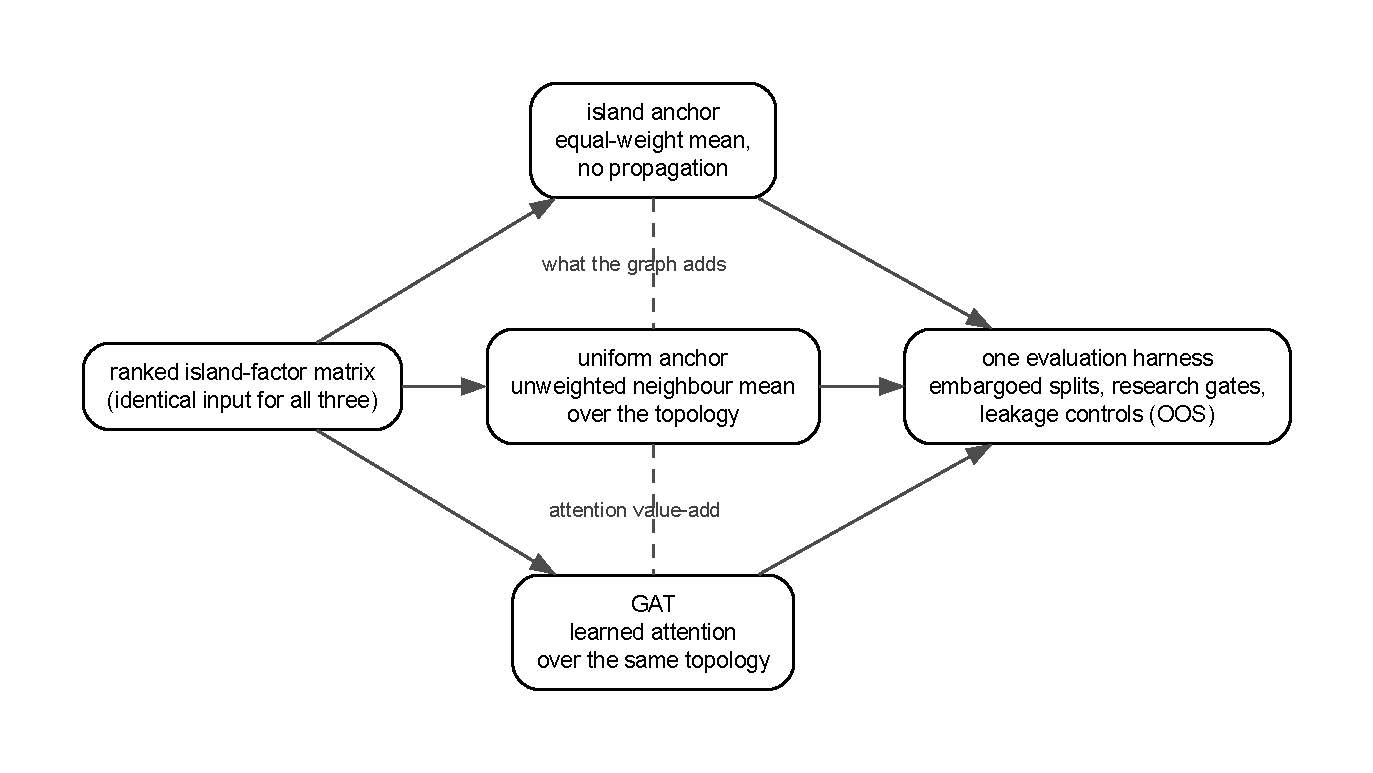
\includegraphics[width=0.88\textwidth]{isolation_anchors.pdf}
  \caption{The attention A/B. All three factor constructions read the
  same ranked island-factor matrix and are scored by the same
  evaluation harness; the two dashed comparisons are the quantities
  this report is about --- what the graph adds (island anchor versus
  uniform anchor) and what learned attention adds (uniform anchor
  versus GAT, the attention value-add).}
  \label{fig:iso-anchors}
\end{figure}

The difference between the GAT's out-of-sample Sharpe and the uniform
anchor's is the \emph{attention value-add}, the quantity the core thesis
stands on. It isolates the contribution of learned attention while
holding the information set and the graph fixed. Where the four gates ask
``is the composite a good factor?'', the A/B asks the sharper question
``did learning the edge weights matter?'' --- and the two questions turn
out to have different answers in \cref{ch:equity}.

\section{Forecast-skill apparatus (energy reframe)}
\label{sec:skill}

After the energy alpha attempt concluded negatively
(\cref{ch:energy}), the energy question was reframed from ``is there a
tradeable cross-sectional signal?'' to ``does the physical
interconnector graph improve forecast accuracy?''. The measurement
apparatus changes accordingly. The metric is a skill score against
persistence,
\[
\text{skill} = 1 - \mathrm{MSE}/\mathrm{MSE}_{\text{persistence}},
\]
scored out-of-sample at $k$ = 24 hours, alongside MAE and the
cross-sectional rank-IC. Persistence (tomorrow equals today) scores zero
by construction; a model must beat carrying yesterday forward to show any
skill at all.

Candidates form a ladder in which each rung isolates one ingredient: a
seasonal-naive rung isolates the diurnal cycle; a per-node ridge
regression on physical drivers (load, wind and solar forecasts, fuel
price) isolates what a zone's own fundamentals add; a ridge with
uniform neighbour averaging isolates what the interconnector graph adds
without learning; and the GAT rungs isolate what learned attention adds
on top. The anchors of \cref{sec:anchors} reappear here in forecasting
form --- the value claim is the margin over the no-graph rung \emph{and}
over the uniform-graph rung, not the absolute skill.

Feature timing follows the day-ahead market's information structure:
load, wind, and solar forecasts for hour $t+k$ are published
before $t$ and may legitimately be used as features for $t+k$; realised
quantities (actual load, generation mix) are known only up to $t$ and
enter as point-in-time anchors. The synthetic negative control carries
over: synthetic zones are generated independently, so the test suite
asserts that the graph rung does not beat the no-graph rung on
synthetic data. Any measured graph lift can then only come from real
cross-zonal coupling.


\chapter{Equity Track: GAT Relational Factors}
\label{ch:equity}

The equity track asks whether propagating island-alpha information over a
correlation graph produces a factor worth having, and --- the sharper
question, RQ1 of \cref{ch:intro} --- whether \emph{learning} the
propagation weights matters. This
chapter reports the experiments in the order they constrained each other:
the controls that license any positive claim (\cref{sec:eq-controls}),
the first real-data run (\cref{sec:eq-first}), the ablation that
attributed its weaknesses (\cref{sec:eq-ablation}), the seed and device
studies that set the reporting discipline (\cref{sec:eq-variance}),
hyperparameter selection under that discipline
(\cref{sec:eq-hp}), and finally what the trained attention actually does
(\cref{sec:eq-attention}). \Cref{tab:equity-summary} states the headline
up front.

\begin{table}[htbp]
  \centering
  \small
  \caption{Equity track headline results (real yfinance data, 49 names, IC loss).}
  \label{tab:equity-summary}
  \begin{tabular}{l>{\raggedright\arraybackslash}p{0.28\textwidth}>{\raggedright\arraybackslash}p{0.30\textwidth}}
    \toprule
    metric & value & note \\
    \midrule
    Gates passed & 3 / 4 & Uniqueness + Consistency + Robustness pass; Value-added fails \\
    Attention value-add & 30/30 seeds positive & vs the uniform anchor (no learned attention) \\
    Composite best-epoch validation IC & 0.0756 & best-by-valid-IC checkpoint selection \\
    Composite OOS Sharpe & 1.42 & vs best single 2.88 (beats 9 of 10 single factors) \\
    Graph & correlation top-k (~50 names + GICS sectors) & estimated backbone (not physical) \\
    Data & real yfinance 2021-01$\to$2026-06 & 49 names; IC loss; 50 epochs \\
    \bottomrule
  \end{tabular}
\end{table}


\section{Controls before claims}
\label{sec:eq-controls}

No positive number in this chapter means anything unless the pipeline can
be shown to find nothing where nothing exists. Three controls establish
this.

First, the synthetic negative control: fifty random-walk price series run
through the full pipeline --- graph construction, training, gates. The
gates correctly report no edge. Value-added and Consistency fail (OOS IC
around $-0.06$, negative Sharpe value-add), while Uniqueness and
Robustness pass, as they should: they measure structural properties of a
factor, not the presence of signal.

Second, the automated pair of controls that runs in the test suite on
every change. Shuffling each snapshot's labels across nodes and retraining
must collapse the validation IC to zero, and it does, for both loss
functions. Planting a recoverable signal --- the label set equal to a
standardised input feature --- must let the same training loop recover it,
and it does. The second half is what makes the first half meaningful: the
IC collapses on shuffled labels because there is nothing to learn, not
because the trainer is broken.

Third, a convergence probe for the training objective itself. On the
planted-signal panel the IC loss recovers the signal essentially
completely (validation IC 0.99 and above at learning rate $10^{-3}$),
where MSE plateaus at 0.33. The IC loss is unstable early at higher
learning rates --- at $5\times10^{-3}$ it bounces near zero for some forty
epochs before converging --- which fixed the default learning rate at
$10^{-3}$ and the IC loss as the default objective.

\section{First real-data run}
\label{sec:eq-first}

The first run on market data used daily bars for the fifty-name universe
(one name, ORCL, failed to download, leaving 49 names, 1{,}364 trading
days and 66{,}836 panel rows spanning January 2021 to June 2026), the ten
island alphas as node features, a static correlation graph built from
data before the split date, and IC-loss training for fifty epochs.

Training behaved like the textbook picture. The training loss fell
monotonically while the validation IC rose to a peak of 0.0756 at epoch
32 and then decayed to 0.0418 by the final epoch --- plain overfitting.
Best-epoch checkpointing therefore deployed the epoch-32 weights; had the
pipeline returned the final epoch, as an earlier version of the code
silently did, the deployed model would have carried barely half the
validation IC. The checkpoint fix paid for itself on its first contact
with real data.

The four gates split three to one. Consistency (score 0.63), Uniqueness
(maximum absolute correlation against any single alpha, 0.257) and
Robustness (0.68) pass; Value-added fails, with a composite OOS Sharpe of
1.42 against 2.88 for the best single island alpha. The honest reading
cuts both ways. The composite is a real, unique, consistent signal ---
the second-best of the eleven factors on the board, beating nine of the
ten singles it was built from, and correlated with none of them above
0.26. It is genuinely new information rather than a repackaging of its
inputs. But the strictest bar --- beat the maximum of ten competitors ---
stayed open here and, as the rest of this chapter shows, never closed.

The run also posed the question that drove the next experiment: the
validation IC of 0.076 decayed to an OOS IC of 0.007 over the roughly
1.6-year OOS window. Was the frozen correlation graph going stale, or the
frozen model weights?

\section{Attributing the decay: graph versus model}
\label{sec:eq-ablation}

A $2\times2$ ablation crossed the graph axis (static, frozen at the split
date, versus dynamic, rebuilt per snapshot from a trailing window) with
the retraining axis (single fit versus walk-forward refits every 63
snapshots). All four cells used one shared data fetch (all fifty names
this time, 68{,}200 rows), the same split, the same seed, and carried the
two no-learning anchors of \cref{sec:anchors}.
\Cref{tab:eq-ablation} shows the result.

\begin{table}[htbp]
  \centering
  \caption{The graph~$\times$~retraining ablation, one seed, IC loss.
  ``Att.\ VA'' is the attention value-add: GAT OOS Sharpe minus the
  uniform anchor's. Anchors, for reference: island mean Sharpe $-2.13$;
  uniform anchor $-1.05$ (static graph) and $-1.19$ (dynamic).}
  \label{tab:eq-ablation}
  \begin{tabular}{lS[table-format=-1.4,round-precision=4]S[table-format=-1.2,round-precision=2]lS[table-format=-1.2,round-precision=2]}
    \toprule
    Configuration & {OOS IC} & {OOS Sharpe} & Gates & {Att.\ VA} \\
    \midrule
    static + single       & -0.0051 &  1.04 & F/F/T/T & +2.09 \\
    dynamic + single      & -0.0348 & -1.01 & F/F/T/T & +0.18 \\
    static + walk-forward & +0.0200 &  1.95 & F/T/T/T & +3.00 \\
    dynamic + walk-forward& +0.0007 &  0.05 & F/T/T/T & +1.24 \\
    \bottomrule
  \end{tabular}
\end{table}

Two findings, one of them negative. Walk-forward retraining is the lever:
it lifts the static-graph cell from an OOS IC of $-0.005$ to $+0.020$ and
flips the Consistency gate to pass. The decay diagnosed in
\cref{sec:eq-first} was model staleness. The dynamic graph, by contrast,
hurts in both arms --- per-snapshot correlation estimates from a trailing
window are noisy, and the frozen train-period graph evidently acts as a
regulariser. This negative result is worth having: the intuitively
appealing refinement (``keep the graph fresh'') makes things worse as
implemented, and the project kept the static graph with its mild,
disclosed in-sample lookahead rather than trade OOS performance for
cosmetic cleanliness.

The attention A/B, meanwhile, is positive in every cell. Both no-learning
anchors are clearly negative out-of-sample; the GAT beats the uniform
anchor by $+0.2$ to $+3.0$ Sharpe on the same topology with the same
inputs, and its scores correlate with the uniform anchor's at Spearman
$-0.29$ to $-0.14$ --- it is not learning to smooth, it is learning
something else. Against the strict value-added bar the best cell still
falls short (best single at 3.07; the gap narrows from $-2.03$ to
$-1.12$), but the core-thesis comparison holds regardless of which cell
one reads.

One warning surfaced here as well: the static+single cell read
$-0.0051$/1.04 where the near-identical first run had read $+0.0066$/1.42.
Run-to-run variance was clearly material, which is what the next section
is about.

\section{Variance: seeds, devices, and the reporting protocol}
\label{sec:eq-variance}

Five seeds per arm on the same panel put numbers on the spread. The
single-fit arm scored an OOS Sharpe of $0.73 \pm 0.25$ (per-seed range
0.36--1.04) and the walk-forward arm $1.15 \pm 0.75$ (range 0.13--1.95);
walk-forward's mean advantage came with three times the variance, and a
Welch $t$ of about 1.2 at $n=5$ per arm. The single-seed reading of the
ablation --- ``walk-forward is the lever'' --- had ridden the luckiest
walk-forward draw. Meanwhile the attention value-add was positive in all
ten runs, spanning $+1.18$ to $+3.00$ Sharpe against a seed-independent
anchor: the core claim survived the variance study; the walk-forward
claim was downgraded to ``improves the mean, adds variance, not
significant at $n=5$''.

A hardware benchmark added an unplanned second lesson. Moving training to
a laptop GPU was 24--32\% \emph{slower} at this graph size --- fifty
nodes and ten features per snapshot is latency-bound, and kernel-launch
overhead dominates --- so production runs stayed on CPU. More
interesting was that the same seed on a different device swung the result
by the full width of the seed distribution. The seed fixes the initial
weights, but dropout masks come from each device's own random stream and
parallel reductions round in a different order, so training diverges from
the first step; a cross-device rerun is another draw from the same
distribution, not the same experiment on new hardware.

Together these fixed the reporting protocol for everything that follows:
every headline number is a mean $\pm$ standard deviation over at least
five seeds on a fixed device, and what the project claims to be
reproducible is the distribution, not bit-exact point estimates.

\section{Hyperparameter selection with clean hands}
\label{sec:eq-hp}

The hyperparameter search was designed so that the OOS window could not
influence selection even in principle. Twenty-four configurations
(learning rate $\{5\times10^{-4}, 10^{-3}, 3\times10^{-3}\}$, hidden size
$\{32, 64\}$, heads $\{2, 4\}$, layers $\{1, 2\}$) ran three seeds each
--- 72 training runs scored exclusively on the double-embargoed
validation IC, with no OOS metric computed anywhere in the grid. Only the
winner then touched the OOS window, once, with fresh seeds.

The grid's surface is flat on top: six configurations sit within
validation IC 0.10--0.115, and the shipped default ranked third. The one
structural regularity is depth --- all six top configurations have two
GAT layers. Results are therefore robust to reasonable hyperparameter
choices, which is simultaneously a robustness point and a caution against
reading much into tuning.

The winner's OOS validation initially produced a finding that did not
survive its own scrutiny. The validation run had silently executed on the
GPU --- the CUDA wheel had just been installed and the fitting routine
auto-selected it --- while the reference numbers it was compared against
were CPU runs. Given the cross-device divergence of
\cref{sec:eq-variance}, that comparison confounded device with
configuration. The code was fixed the same day (CPU is now an explicit
default, CUDA opt-in) and the validation rerun on CPU. The deconfounded
result: in the single arm the winner is a wash against the default (0.80
vs.\ 0.73 Sharpe, IC near zero in both), but in the walk-forward arm it
is better on the mean and far tighter --- OOS IC $0.0148 \pm 0.0043$
against the default's $0.0055 \pm 0.0147$, a 2.7-fold mean with a third
of the variance, all five seeds positive on both IC and Sharpe, and the
IC mean 3.4 standard deviations above zero. Within this configuration,
walk-forward versus single reaches significance (Welch $t \approx 3.9$ on
IC, $\approx 2.4$ on Sharpe at $n=5$ per arm), upgrading the walk-forward
claim to ``significant in the tuned configuration, directionally
consistent everywhere''.

The best known setup is therefore the static graph, IC loss,
walk-forward refits, and the winner hyperparameters, at an OOS IC of
$0.0148 \pm 0.0043$ and OOS Sharpe of $1.37 \pm 0.39$. Across the three
run families --- seed study, GPU validation, CPU rerun --- the attention
value-add is positive in 30 of 30 seeded runs, spanning $+0.69$
to $+3.03$ Sharpe. That, not any single point estimate, is the equity
track's central result.

\section{What the attention learned}
\label{sec:eq-attention}

The A/B says learned attention beats uniform averaging; attention
analysis on a representative trained model (919{,}336 edge-weight rows
over 1{,}364 dates) says how.

The attention is genuinely relational. The mean self-loop weight is
0.084 --- the model places 91.6\% of its attention mass on neighbours ---
which rules out the trivial failure mode in which attention collapses
onto each node's own features and the graph is decoration. But across a
node's roughly 12.5 neighbours the distribution is nearly uniform:
normalised entropy 0.956, a top-neighbour share of 0.152 where exact
uniformity would give 0.08, and a sector-homophily lift of just $+0.019$
(attention-weighted same-sector share 0.330 against a structural 0.311).
The trained model is a gentle reweighting of mean pooling, not a sharp
selector. This is the mechanism behind the whole chapter: small, learned
tilts on top of broad pooling explain why the GAT's edge over the uniform
anchor is consistent yet modest, and why its scores are nearly
uncorrelated with the anchor's.

The coarse structure is also temporally stationary: the self/neighbour
split holds at 0.91--0.92 and the homophily lift stays within
$+0.01$ to $+0.03$ across the full 2021--2026 span, with no visible break
at the IS/OOS boundary (\cref{fig:att-neighbour}). The project's original design hypothesis --- that
attention would adapt to macro regimes --- is not supported at this
aggregate level, and the report states so; whatever adaptation exists
lives in per-name weights inside a stable coarse structure. Finally, the
names drawing the most incoming attention are mega-caps and sector
bellwethers --- AMZN, NFLX, AVGO, GS, CAT, NVDA, MSFT, LIN --- exactly
the names the rest of the universe co-moves with, a qualitative validity
check the attention passes.

\begin{figure}[htbp]
  \centering
  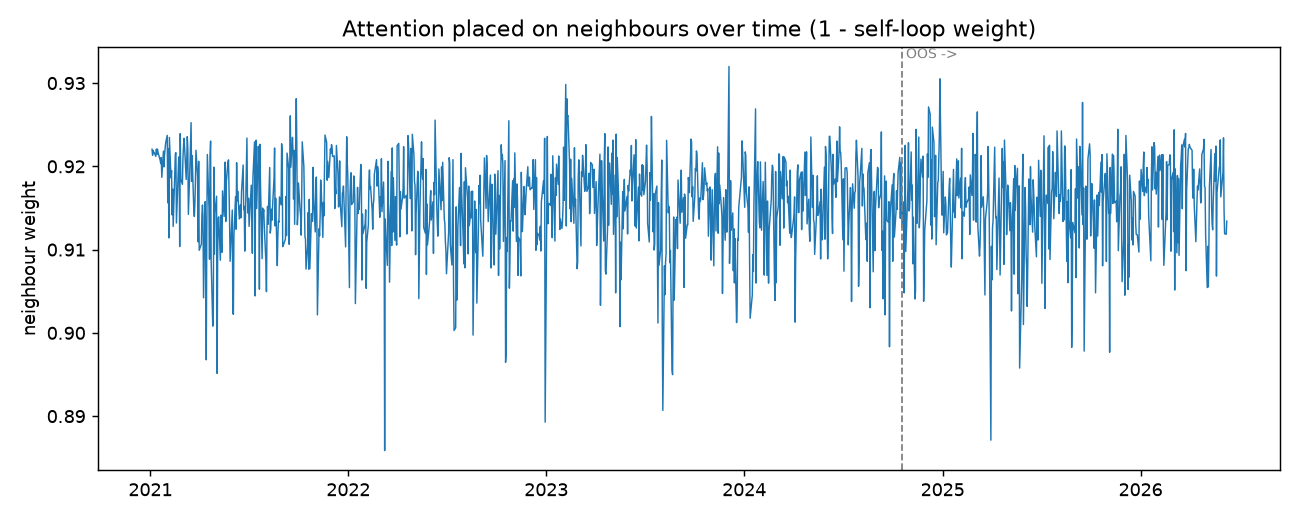
\includegraphics[width=\textwidth]{att_neighbour_weight.png}
  \caption{Attention mass placed on neighbours (one minus the
  self-loop weight) per snapshot over 2021--2026, from the archived
  attention analysis of the representative trained model. The share
  stays in a narrow band around 0.91--0.92, with no break at the
  dashed IS/OOS boundary --- the stationarity reported in the text.}
  \label{fig:att-neighbour}
\end{figure}

\section{Summary of the equity evidence}
\label{sec:eq-summary}

Learned attention over the correlation graph reliably beats unlearned
propagation over the same graph with the same inputs: positive attention
value-add in 30 of 30 seeded runs across two hyperparameter
configurations and two devices. The resulting composite is a real,
unique, consistent factor that beats nine of its ten inputs but not the
best of them; the value-added gate remains the one honest failure.
Dynamic graphs hurt, walk-forward retraining helps (significantly so in
the tuned configuration), single-seed and single-device numbers are not
to be trusted, and the attention mechanism itself is interpretable ---
relational, nearly uniform, stationary, and centred on economically
sensible hubs.

\chapter{Energy Track: From Alpha to Forecasting}
\label{ch:energy}

The energy track set out to repeat the equity result on a physically
grounded graph: twenty European bidding zones connected by the actual
cross-border transmission network, with day-ahead spot prices from the
ENTSO-E Transparency Platform \cite{entsoe-tp}. \Cref{fig:interconnector}
shows that graph as configured in the repository --- twenty zones, 38
physical borders and HVDC links, reference data rather than anything
estimated from prices. The track ended somewhere more
interesting than its plan. The cross-sectional alpha framing failed --- not quietly,
but through three nested evaluation artifacts, each of which initially
produced spectacular numbers and each of which the project's own controls
caught (\cref{sec:en-negcontrol,sec:en-artifact,sec:en-redesign,sec:en-clip}).
The track was then reframed as a forecasting problem, where the graph
finally showed genuine, control-validated value, concentrated exactly
where relational structure should matter most: on cross-border spreads
(\cref{sec:en-forecast,sec:en-edge}). This chapter reports the arc in
order, because the order is the contribution. Two research questions run
through it: whether one kernel transfers to a physical graph without
manufacturing false positives (RQ2), and whether that graph improves
forecasts (RQ3).

\begin{figure}[t]
  \centering
  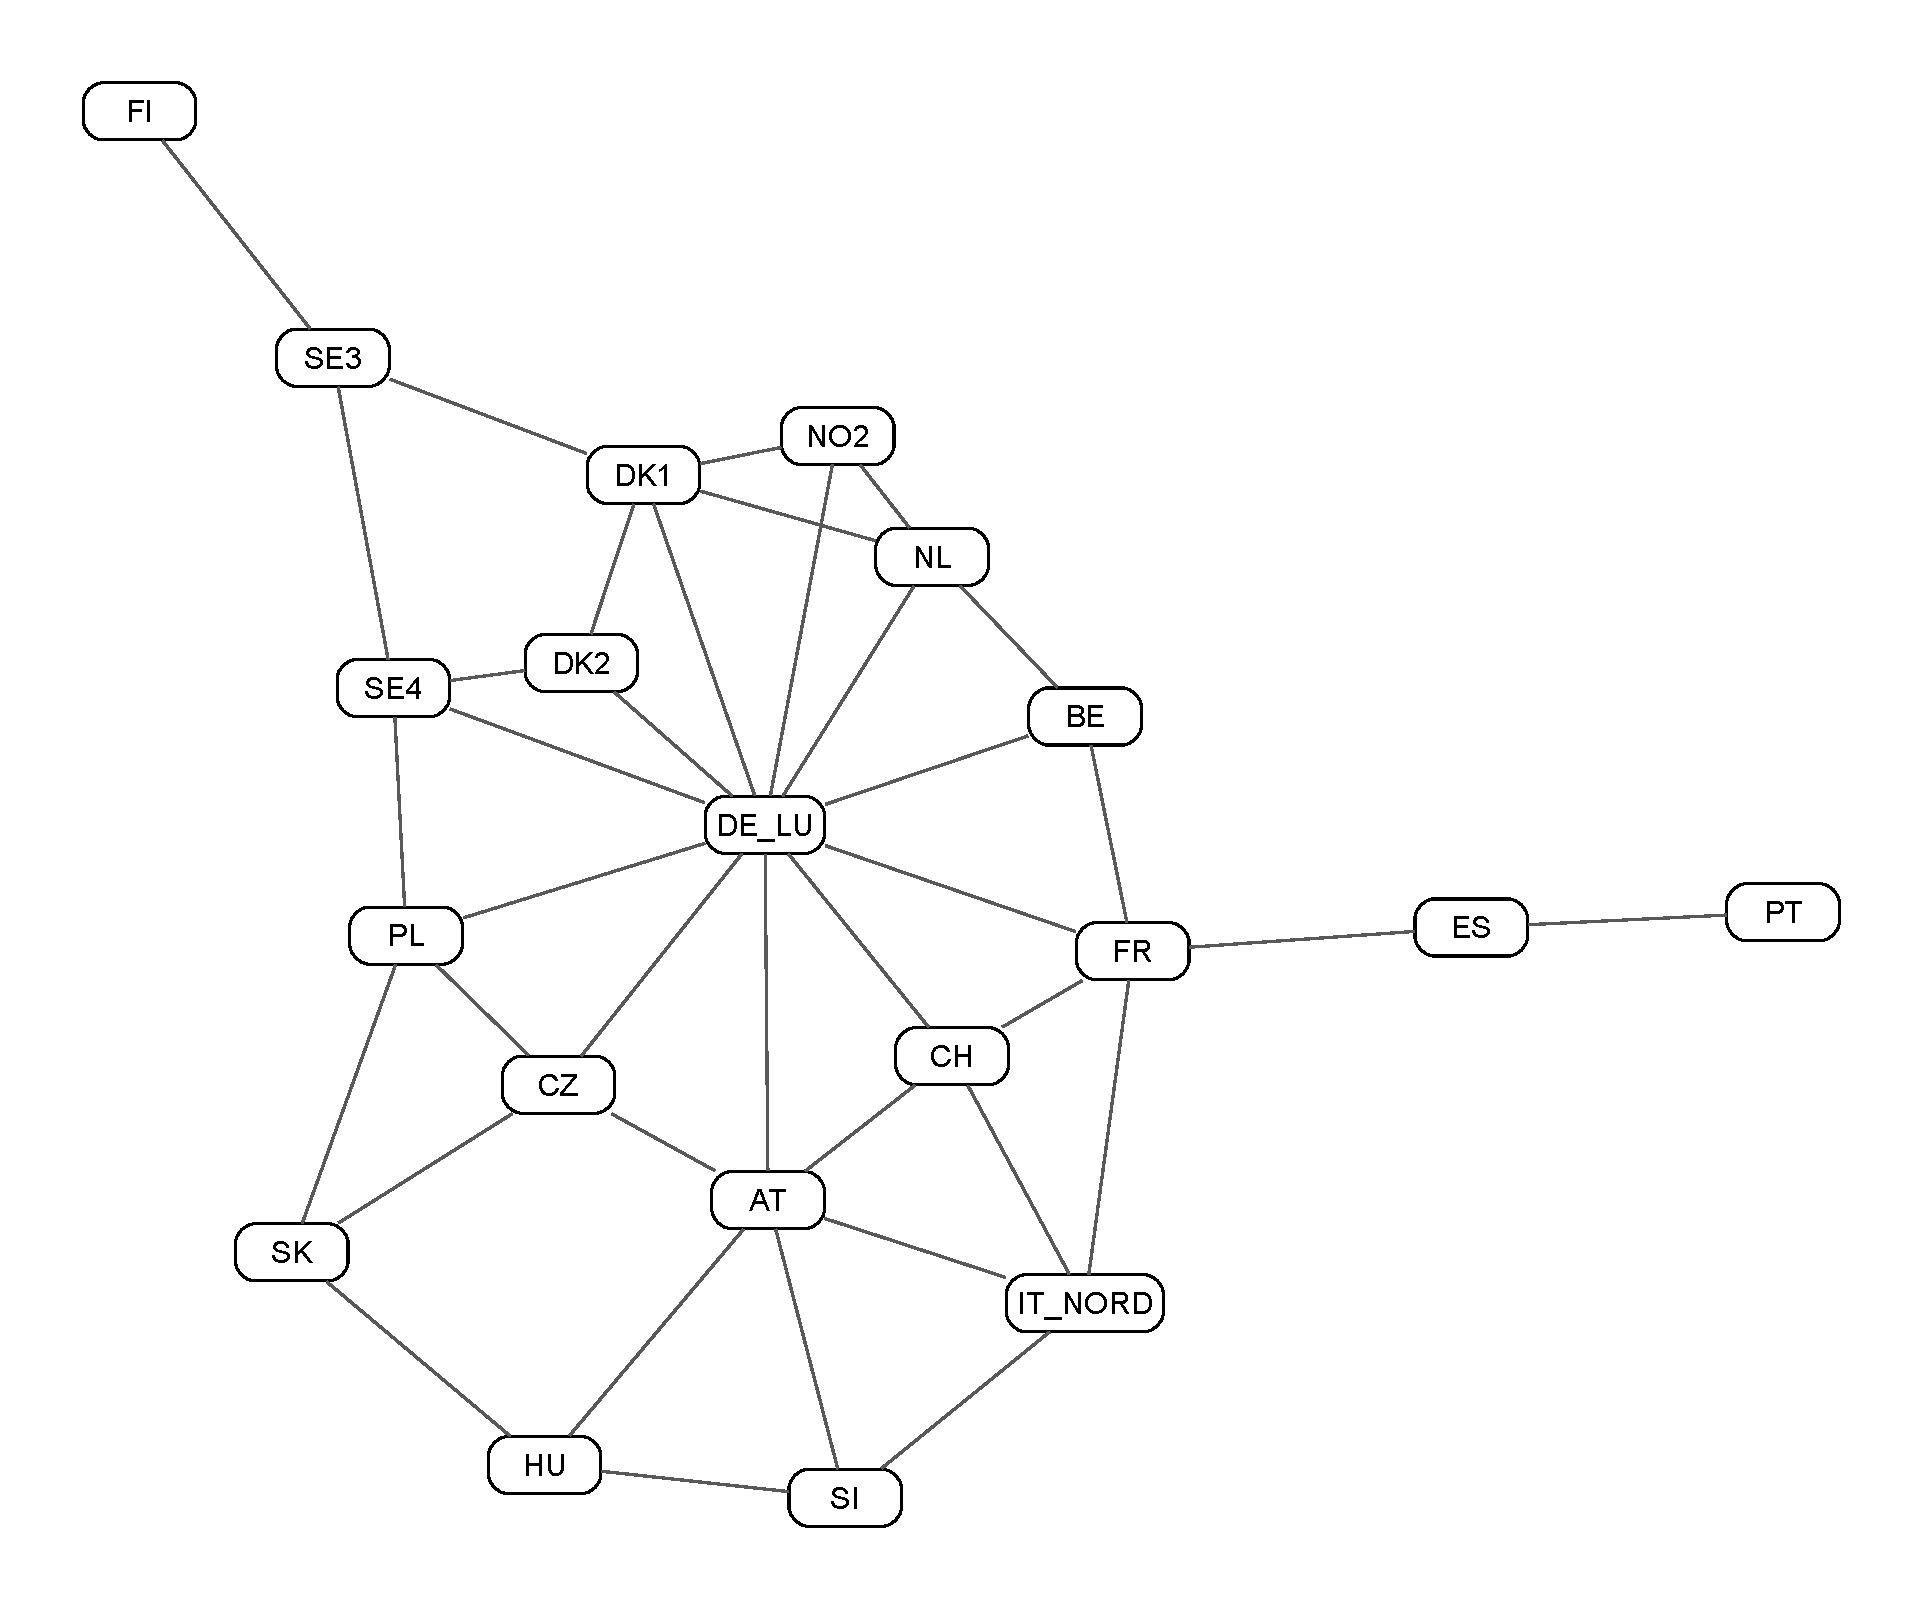
\includegraphics[width=0.78\textwidth]{interconnector.pdf}
  \caption{The energy graph: 20 European bidding zones and their 38
  physical cross-border interconnections (land borders and HVDC
  cables), drawn from the repository's reference data. Unlike the
  equity correlation graph, nothing here is estimated --- the topology
  is the grid. DE\_LU, with eleven interconnectors, is the network's
  natural hub.}
  \label{fig:interconnector}
\end{figure}

\section{One kernel, two graphs --- and a second negative control}
\label{sec:en-negcontrol}

The dual-track design goal was engineering economy: the equity GAT, its
training loop, its four gates, and its A/B anchors run unchanged on the
energy panel; only the graph (physical interconnectors instead of
estimated correlations), the label horizon (24 hours instead of 5 days),
and the node set (bidding zones instead of symbols) differ. That goal was
met literally --- the same kernel functions are called by both tracks ---
and the first energy run doubled as a control.

On synthetic power data (2{,}857 hourly snapshots, 57{,}140 rows,
generated without any cross-zonal coupling) the pipeline correctly finds
nothing: OOS IC around $-0.01$ in both retrain arms, and, crucially, the
attention value-add is \emph{negative} ($-0.74$ single, $-0.59$
walk-forward). When there is no relational signal, the GAT is worse than
uniform neighbour averaging, not better. This is the energy analogue of
the equity negative control, on a structurally different graph: even a
learned attention layer over a physical topology does not manufacture
signal from noise.

\section{Real data, implausible result}
\label{sec:en-artifact}

The live ENTSO-E run covered all twenty zones for the full year 2024 at
hourly resolution --- 175{,}200 rows, with every configured zone
returning data. Real power prices immediately justified the label's
engineering: they spanned $-427$ to $1{,}896$~EUR/MWh, negative in 3.95\%
of hours. The pipeline ran end to end without kernel changes. The
numbers it produced were an OOS IC of 0.20, an OOS Sharpe of 8.25, a
composite roughly one hundred times its best single input, and four
gates out of four.

The same kernel earns a Sharpe of about 1.4 on equities. A result this
much better is not a discovery; it is a symptom. Diagnosis found three
compounding artifacts. First, overlapping labels: a 24-hour forward
return sampled hourly gives consecutive observations that share 23 of
their 24 hours --- measured lag-1 autocorrelation 0.91 --- while the
Sharpe computation treats them as independent, understating the
denominator by an order of magnitude. Second, the ``signal'' is trivial:
a one-line predictor, the negative of the current spot price, scores a
cross-sectional IC of 0.235, \emph{higher} than the GAT's 0.20. Whatever
the model learned, it is dominated by deterministic diurnal
mean-reversion. Third, the annualisation constant was the equity one
(252 periods per year) applied to hourly data (8{,}760). On top of all
three sits a market-structure lookahead: the day-ahead auction publishes
all 24 hours of day $D$ at once on $D-1$, so an ``hourly'' 24-hour-ahead
label is partly contemporaneous information.

The point the report wants to preserve is that the magnitude itself was
the alarm. The same scepticism that made the synthetic controls a design
feature flagged the real-data number as not credible, rather than
publishing a Sharpe of 8.

\section{Redesign in the day-ahead frame}
\label{sec:en-redesign}

The redesign moved the evaluation to the market's actual decision
frequency. The day-ahead auction clears once per day, so the snapshot
became the delivery day: base-load-aggregated features from data up to
day $D$, a label equal to the genuinely-unknown next-day base-load price
change $D \to D{+}1$, non-overlapping by construction, annualised at 365.

The mechanical checks all came back clean. Label lag-1 autocorrelation
fell from 0.91 to $-0.10$; the shuffle-label control gave a validation IC
of 0.07 against 0.19 for real labels, so the remaining signal is not
leakage. And yet the result stayed implausible: GAT composite OOS Sharpe
11.08 --- with the trivial negative-price predictor at 6.15. The
interim reading was that the pipeline was now honestly measuring a real
but non-tradeable physical regularity: the law of one price across
interconnected zones, already priced by cross-border capacity auctions.
That reading was half right, and its other half is the most instructive
result in this report.

\section{The third artifact: a clip on the evaluation return}
\label{sec:en-clip}

A direct challenge --- \emph{have you actually confirmed the strategy
would lose nothing?} --- prompted one more check: recompute the same
strategies under different definitions of the evaluation return.
\Cref{tab:en-clip} shows what that found.

\begin{table}[htbp]
  \centering
  \caption{The return-definition diagnostic (real ENTSO-E daily frame,
  OOS). The $\pm0.8$ clip, inherited from the training label, was also
  applied to the evaluation return in E13 --- and manufactured the
  entire positive result.}
  \label{tab:en-clip}
  \begin{tabular}{lS[table-format=-2.2]S[table-format=-2.2]}
    \toprule
    Evaluation return & {trivial $-$price Sharpe} & {GAT Sharpe} \\
    \midrule
    floored + $\pm0.8$ clip (as trained) & +6.28 & +11.00 \\
    winsorised $\pm0.5$                  & +4.61 & {---}  \\
    log return                           & +3.75 & {---}  \\
    plain relative return (honest)       & -1.52 & -1.54  \\
    \bottomrule
  \end{tabular}
\end{table}

The mechanism is specific and worth stating plainly. The long-short
strategy shorts expensive zones. European power prices have fat right
tails --- scarcity spikes reaching $1{,}896$~EUR/MWh in this sample ---
and the $\pm0.8$ clip on the evaluation return caps exactly those
short-leg losses. Removing the clip turns a Sharpe-11 winner into a
strategy that loses money, for the GAT and the one-line baseline alike.
The rank-IC, meanwhile, stays at about 0.21 under both return
definitions: cheap zones really do tend to rise relative to expensive
ones, but ranking correctly is blind to tail magnitudes, and the tails
are where this strategy's money is lost. A positive IC coexisting with
negative PnL is the transferable lesson --- never transform the
evaluation return, and never read rank quality as profitability. The
equity track is unaffected: its evaluation return was never clipped.

The final verdict on the energy alpha question is therefore airtight and
negative. Under honest returns the day-ahead cross-sectional strategy
loses money (Sharpe about $-1.5$); every positive energy number along the
way was an artifact --- overlap, annualisation, then the return clip ---
and the GAT adds no tradeable value over a one-line baseline. The fix
(evaluation on unclipped returns) shipped as the default, so the
repository can no longer reproduce the inflated numbers.

\section{The reframe: does the graph improve forecasts?}
\label{sec:en-forecast}

What survives E13b is a genuine question the data can answer: not ``is
there alpha?'' but ``does the interconnector graph improve forecast
skill?'' --- measured with the ladder of \cref{sec:skill} on six months
of real ENTSO-E data (20 zones, 87{,}360 rows, with day-ahead load, wind
and solar forecasts, realised load, and generation mix as drivers).
\Cref{tab:energy-node-skill} shows the node-level ladder, and
\cref{fig:energy-ladder} draws it with one added ingredient per rung.

\begin{table}[htbp]
  \centering
  \small
  \caption{Node-level price forecast skill ladder (skill $=1-\mathrm{MSE}/\mathrm{MSE}_{\mathrm{persistence}}$, OOS, $k=24$h).}
  \label{tab:energy-node-skill}
  \begin{tabular}{lll>{\raggedright\arraybackslash}p{0.34\textwidth}}
    \toprule
    predictor & skill & rank ic & note \\
    \midrule
    persistence & 0.000 & 0.637 & reference (tomorrow = today) \\
    seasonal\_naive & 0.000 & 0.637 & diurnal carry \\
    no\_graph\_ridge & 0.224 & 0.636 & own physical drivers (ridge) \\
    uniform\_graph\_ridge & 0.355 & 0.584 & + interconnector-neighbour mean (unlearned graph) \\
    gat\_node & 0.347 & 0.612 & learned attention (PyG GATv2; 5-seed mean) \\
    gat\_congestion & 0.346 & 0.615 & + price-spread congestion edge feature (5-seed mean) \\
    \bottomrule
  \end{tabular}
\end{table}


\begin{figure}[htbp]
  \centering
  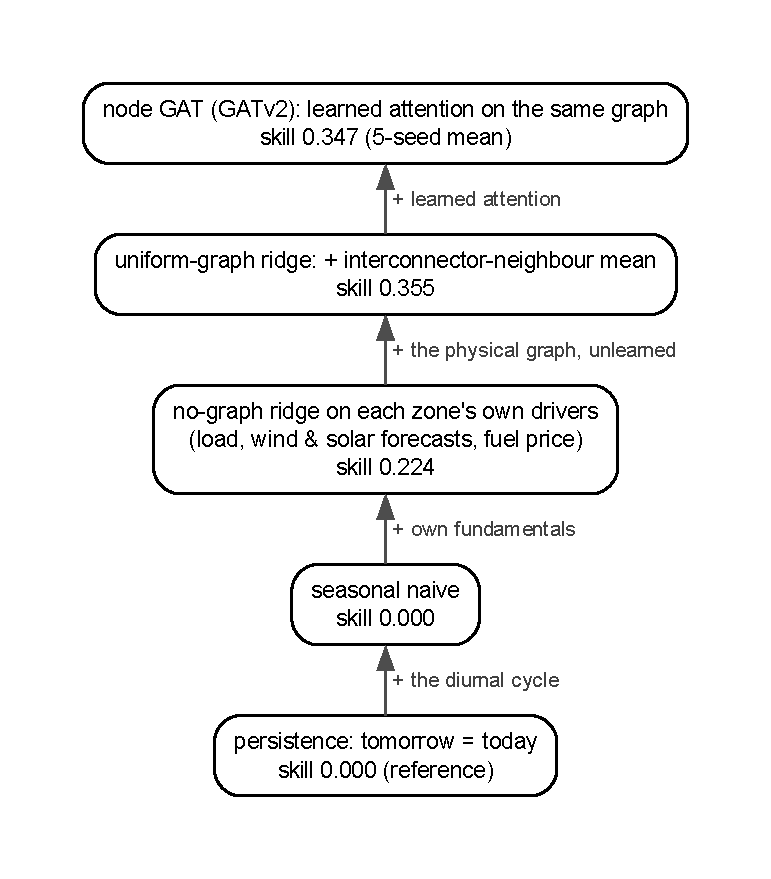
\includegraphics[width=0.54\textwidth]{energy_ladder.pdf}
  \caption{The node-level forecast ladder of
  \cref{tab:energy-node-skill}, drawn as a ladder. Each rung adds
  exactly one ingredient, so each skill increment isolates one cause.
  The published drivers enter at the ridge rung and are shared by every
  rung above it; the graph's contribution ($+0.131$) enters below any
  learning.}
  \label{fig:energy-ladder}
\end{figure}

Three findings, in decreasing order of robustness. First, the graph
carries real forecast value: uniform neighbour averaging over the
interconnector topology lifts skill by $+0.131$ over the no-graph ridge
with the same drivers. The synthetic negative control (independent
zones) shows no such lift, so the gain is genuine cross-zonal coupling.
This rung is pure numpy --- no learned model is involved --- which makes
it the hardest number in the chapter to argue with.

Second, learned attention beats the uniform anchor on cross-sectional
\emph{ranking} in five seeds of five (rank-IC 0.61 against 0.58) but is
a wash on MSE skill (better in two seeds of five). Uniform
neighbour-averaging turns out to be near MSE-optimal on this graph --- a
hard bar --- so the GAT's robust edge here is order, not magnitude,
echoing the equity finding that attention's value is a modest tilt on
broad pooling.

Third, the congestion hypothesis --- that attention should down-weight
saturated borders if told how congested they are --- is not supported.
Two operationalisations of the edge feature were tried: the current
cross-border price spread (a leak-safe proxy), and ground-truth physical
flows over day-ahead transfer capacity fetched for all 38 borders. The
proxy's apparent gain existed only in a hand-rolled dense GAT
implementation ($+0.031$ skill, five of five seeds) and vanished under
the standard PyG GATv2 ($-0.002$, two of five); the ground-truth version
beat node-only attention in one seed of five. The hypothesis is not
refuted --- capacity data covered only 36\% of borders, and the most
coupled region uses flow-based coupling that a flow-over-capacity ratio
cannot express --- but as a smooth additive edge feature, congestion
does not add forecast skill. The two-backend check deserves its
methodology note: a single-seed PyG run had initially shown $+0.072$, a
lucky draw that a five-seed rerun corrected, and the cross-implementation
comparison is what stopped a fragile effect from becoming a claim.

\section{Edge-level spread prediction: the relational payoff}
\label{sec:en-edge}

The last experiment moved the target instead of the model. A
cross-border price spread $\mathrm{spot}_a - \mathrm{spot}_b$ is
irreducibly relational --- it does not exist for a single node, and it is
the object that transmission rights actually price. A GAT computes node
embeddings by message passing over the interconnector graph; a small MLP
head predicts each border's next-day spread from the two endpoint
embeddings and the current spread. The baseline that matters is a ridge
that already sees both endpoints' drivers and the current spread ---
so any gain over it is whole-network context, not information the
baseline lacks. \Cref{tab:energy-edge-skill} shows the ladder over the
38 borders.

\begin{table}[htbp]
  \centering
  \small
  \caption{Edge-level cross-border spread prediction (38 borders, OOS, $k=24$h, 5-seed means).}
  \label{tab:energy-edge-skill}
  \begin{tabular}{lll>{\raggedright\arraybackslash}p{0.34\textwidth}}
    \toprule
    predictor & skill & rank ic & note \\
    \midrule
    edge\_persistence & 0.000 &  & spread today (reference) \\
    edge\_ridge & 0.192 & 0.67 & both endpoints' day-ahead drivers + current spread (no graph) \\
    edge\_gat & 0.248 & 0.68 & GAT node embeddings $\to$ edge MLP head (message passing; 5-seed mean) \\
    \bottomrule
  \end{tabular}
\end{table}


The edge GAT beats the both-endpoint ridge by $+0.056$ skill --- about
29\% relative --- in five seeds of five, and the synthetic control
inverts as it should: on independent zones the same architecture is
\emph{worse} than the ridge, so the real-data gain is structure, not
capacity. This is the project's strongest relational result, and its
placement is the point: node-level price forecasting barely needed the
graph, congestion-as-edge-feature was null, and the GNN's value
concentrates precisely on the target that cannot be defined without the
relation. Caveats stated once: a single six-month window, untuned
hyperparameters, and modest absolute skill --- spreads are noisy
differences.

\section{Summary of the energy evidence}
\label{sec:en-summary}

\begin{table}[htbp]
  \centering
  \small
  \caption{Energy forecasting track: what is and is not supported (real ENTSO-E data, 20 zones, 5-seed means).}
  \label{tab:energy-findings}
  \begin{tabular}{>{\raggedright\arraybackslash}p{0.24\textwidth}>{\raggedright\arraybackslash}p{0.22\textwidth}lll}
    \toprule
    finding & comparison & skill delta & seeds & verdict \\
    \midrule
    Graph helps price level & uniform - no-graph & +0.131 & control-validated & robust \\
    Attention vs uniform (ranking) & gat rank\_ic - uniform & +0.031 & 5/5 & robust \\
    Attention vs uniform (skill) & gat - uniform & -0.008 & 2/5 & wash \\
    Congestion edge feature (price-spread proxy) & gat\_congestion - gat\_node & -0.002 & 2/5 & null \\
    Congestion edge feature (real flow/NTC) & flow - node & -0.005 & 1/5 & null \\
    Edge-level spread (message passing) & edge\_gat - edge\_ridge & +0.056 & 5/5 & robust * \\
    \bottomrule
  \end{tabular}
\end{table}


\Cref{tab:energy-findings} condenses the track. As an alpha project the
energy track concluded negatively three artifacts deep, and the honest
number --- the strategy loses money --- is stated as the finding it is.
As a forecasting project it produced two robust, control-validated
positives (the graph lift of $+0.131$ at node level; the edge-level
message-passing gain of $+0.056$, five of five seeds) and one clean null
(congestion edge features, under both operationalisations). As
methodology it produced the report's most transferable lessons: evaluate
on untransformed returns, distrust magnitudes that outrun their
plausibility class, and require cross-implementation replication before
believing a learned effect.

\chapter{Discussion}
\label{ch:discussion}

Every limitation below is a deliberate scope choice or a measured
finding, not an oversight discovered in retrospect; several are results
in their own right. This chapter names each threat to validity in the
standard vocabulary and states where the project mitigated it, and where
it simply lives with it.

\paragraph{Look-ahead bias.} The report contains a full worked example
of this threat rather than merely a disclaimer: the energy track's first
real-data result (\cref{sec:en-artifact}) was look-ahead bias in two of
its three layers, and the diagnostic arc that dismantled it is the
chapter. On the equity track one mild instance is disclosed and
retained: the static correlation graph is built from data up to the
split date, so early \emph{training} snapshots see a graph estimated
partly from their own future. The out-of-sample window is unaffected ---
the graph strictly predates it --- and the clean alternative, the
dynamic graph, was rejected because it performs worse
(\cref{sec:eq-ablation}). Disclosure was chosen over a cosmetic fix that
costs real out-of-sample performance.

\paragraph{Survivorship bias.} The equity universe is roughly fifty
hand-picked, currently listed US large caps fetched from a free vendor.
Names that failed or delisted over 2021--2026 are absent, which inflates
the absolute level of every Sharpe in \cref{ch:equity}. The core claim
is deliberately insulated: the attention A/B compares models on the
\emph{same} biased universe, so the bias raises both sides of the
comparison rather than manufacturing the gap. Absolute levels should be
read as optimistic; relative margins are the load-bearing numbers. A
survivorship-bias-free vendor is the single highest-value data upgrade a
successor project could make.

\paragraph{Overfitting and data snooping.} Ten alphas, one composite,
and repeated evaluation on one out-of-sample window invite snooping; the
four gates exist to police exactly this, and the hyperparameter search
was designed so the out-of-sample window could not influence selection
(\cref{sec:eq-hp}). The residual risks are stated rather than waved
away: the walk-forward advantage is significant only within the tuned
configuration ($n=5$ per arm) and is otherwise a directional claim; the
flat hyperparameter surface cuts both ways, as robustness and as a
warning that tuning gains here are mostly noise; and the energy
forecasting results rest on a single six-month window with untuned
hyperparameters. The two synthetic negative controls and the
shuffle-label control (\cref{sec:eq-controls,sec:en-negcontrol}) are the
strongest argument that the pipeline as a whole does not snoop.

\paragraph{Transaction costs and tradability.} No result in this report
is net of costs: there is no fill model, no spread, no market impact.
The equity Sharpe of 1.37 is a paper Sharpe on daily bars, and a
five-day-horizon long-short over fifty names would face real turnover
costs. The energy track makes the point more brutally --- its strategy
loses money \emph{before} any costs are applied
(\cref{sec:en-clip}), and the E13b lesson (rank quality does not imply
profitability when tails carry the money) would only sharpen under a
cost model. The platform's stated production boundary
(\cref{sec:pl-layers}) is consistent with this: nothing here is a
trading system.

\paragraph{Regime dependence and external validity.} All equity claims
rest on a single 5.5-year window of one market regime, at one horizon
($k=5$ days), on one universe; all energy forecasting claims on six
months of one calendar year, at one horizon ($k=24$ hours), on twenty
zones. The attention analysis itself argues against over-generalising:
the learned structure is temporally stationary
(\cref{sec:eq-attention}), so the project's own evidence says the model
found a stable statistical regularity, not a regime-adaptive mechanism.
Whether either result survives a different half-decade is untested.

\paragraph{Reproducibility.} What is reproducible is the distribution,
not the point: the same seed produces different results on different
devices, for identified mechanical reasons (\cref{sec:eq-variance}).
All headline numbers are therefore means over at least five seeds on a
fixed device, the test suite pins the leakage-critical logic, and the
archived per-run artifacts allow every table in this report to be
regenerated. Bit-exact cross-device replication is not claimed and, on
CUDA, not attainable.

\paragraph{The open gate.} The relational composite never beat the best
single island alpha --- an OOS Sharpe of roughly 1.4 against roughly 3
--- and this report resists the temptation to soften that bar
post hoc. Two softer readings are available and honestly labelled as
softer: the composite beats nine of its ten inputs, and it is nearly
uncorrelated with all of them (maximum 0.26), which for a practitioner
suggests portfolio value that the max-of-singles gate does not measure.
A marginal-contribution-to-a-multifactor-portfolio reading is the
natural next evaluation, planned but not executed within this project's
scope.

\chapter{Conclusion and Future Work}
\label{ch:conclusion}

The three research questions of \cref{ch:intro} can now be answered
directly.

\emph{Does learned attention add value over unlearned relational
propagation?} On the equity track, yes, with unusual consistency for a
result in this domain: positive attention value-add in thirty of thirty
seeded runs, across two hyperparameter configurations and two devices,
against an anchor that shares the model's inputs and topology. The
mechanism is modest and now understood --- a stationary, near-uniform
reweighting of neighbour pooling --- and the resulting composite is a
real, unique, consistent factor that nevertheless does not beat the best
single alpha it was built from. On the energy forecasting track the
answer is narrower: attention improves cross-sectional ranking over the
uniform anchor in five of five seeds but not mean-squared skill, where
uniform pooling is already near-optimal.

\emph{Does one kernel transfer across heterogeneous graphs without
manufacturing false positives?} Yes, and the negative controls are the
evidence: the same code that finds a consistent positive margin on real
equity data finds nothing on synthetic random walks, finds nothing on
synthetic uncoupled power zones, and --- when real energy data produced
numbers too good to be true --- the surrounding discipline treated the
magnitude as an alarm rather than a result. The transfer claim is
literal: one model class, one training loop, one gate suite, two
structurally different graphs.

\emph{Does the physical topology improve forecasts?} Yes, where it
should. The interconnector graph lifts node-level price forecast skill
by $+0.131$ over an identically-informed no-graph baseline, and the
clearest relational gain sits on the irreducibly relational target:
edge-level spread prediction beats a both-endpoint baseline by $+0.056$
skill in five of five seeds, while a synthetic control inverts the
comparison. Congestion as an explicit edge feature added nothing robust
under either of two operationalisations --- an honest null.

Beyond the questions it set out to answer, the project's most
transferable output is methodological: evaluate on untransformed
returns; treat rank correlation and profitability as different claims;
treat implausible magnitudes as alarms; require seeds, fixed devices,
and cross-implementation replication before believing a learned effect;
and keep negative controls running permanently, because they are what
give positive results their meaning.

\section*{Future work}

Four directions follow directly from the open ends documented in the
experiment log and forecasting notes, in decreasing order of expected
value. First, data: a survivorship-bias-free equity vendor would turn
the biased absolute Sharpe levels into defensible ones, and longer,
multi-window energy samples would test the six-month forecasting results
out-of-sample in time. Second, evaluation: the value-added gate deserves
its portfolio-level variant --- the marginal contribution of the
composite to a multifactor portfolio --- alongside the max-of-singles
bar it never cleared. Third, the forecasting track is untuned: a
hyperparameter grid, seed ensembles, and walk-forward retraining, all
already built for the alpha track, transfer mechanically; an edge-level
congestion target (not just the spread) is the natural next prediction
problem. Fourth, the congestion hypothesis remains open rather than
dead: the flow-based-coupling regions publish shadow prices on critical
network elements, and a congestion signal built from those --- rather
than from flow-over-capacity ratios with partial coverage --- is the
experiment this project would run next. Any renewed energy \emph{alpha}
attempt, by contrast, should wait for genuinely tradeable targets:
balancing or intraday spreads, or transmission-rights-aware profit
accounting.

The report closes where it began. The coupling structure of markets is
information; on the evidence here, learning how to read it earns a
consistent but modest premium over reading it naively, and the
discipline required to measure that premium honestly --- anchors,
controls, embargoes, seeds, and the willingness to let three spectacular
numbers die --- is itself the result this project most confidently
recommends to its successors.


\chapflowfalse
\printbibliography

\appendix
\chapter{Reproducibility}
\label{app:repro}

Everything claimed in this report can be regenerated from the
repository.\footnote{\url{https://github.com/witold-andelie/quant-foundation-gat}}
This appendix records the environment, the commands, and the
mapping from experiment to archived artifact.

\section*{Environment}

Python 3.13 with \texttt{torch 2.12.0} and \texttt{torch\_geometric}
(installed via the project's \texttt{[gnn]} extra); \texttt{PYTHONPATH}
set to \texttt{src}. All headline experiments ran on CPU --- a
deliberate choice after the device study of \cref{sec:eq-variance} ---
with the device recorded per experiment. The equity track fetches
market data through \texttt{yfinance}; the energy track runs on the
synthetic generator by default and on live ENTSO-E data when an API
token is supplied via the \texttt{ENTSOE\_API\_KEY} environment
variable. The warehouse and marts require \texttt{duckdb},
\texttt{dbt-core}, and \texttt{dbt-duckdb}; the GAT pipeline itself does
not.

\section*{Tests}

The full suite is 115 tests; 55 of them cover the capstone modules
(graph construction, training primitives, propagators, factor
providers, both track runners, attention analysis, and the leakage
controls). The leakage controls --- shuffle-label negative control and
planted-signal positive control --- are pinned to CPU for determinism
and run on every change. \texttt{py -m pytest} from the repository root
executes everything.

\section*{Experiments and artifacts}

Each experiment entry in the log (\texttt{docs/gat\_experiment\_log.md},
entries E1--E14) names its run script and its archived outputs. The run
scripts are one-off drivers kept in an untracked scratch area outside
the published repository; each log entry records the configuration they
ran --- model variant, seeds, hyperparameters, device --- and the CLI
commands below drive the same pipelines. The outputs --- per-run
diagnostics, matrix, seed, hyperparameter-grid, winner-validation,
energy, and attention CSV/JSON files, plus five attention figures ---
are date-prefixed under \texttt{docs/results/}. The canonical trained
equity weights are tracked at
\path{data/warehouse/gat_equity.pt}. Every quantitative table in
this report is generated mechanically from those archived CSVs; no
result number in the text was typed by hand from memory.

\section*{Command reference}

The equity pipeline:
\begin{verbatim}
quant-alpha gat-equity --graph {static,dynamic}
                       --retrain {single,walk-forward}
                       --loss {ic,mse}
                       --device {cpu,cuda,auto}
                       --persist
\end{verbatim}
runs end to end and, with \texttt{--persist}, writes the four warehouse
tables of \cref{sec:pl-loop}. The energy alpha runner is
\texttt{run\_gat\_energy} (synthetic or \texttt{source="entsoe"}); the
forecasting ladder is \texttt{quant-alpha energy-forecast --source
\{synthetic,entsoe\} --k 24} with a \texttt{--raw-path} Parquet cache
for repeatable real-data runs. The marts rebuild with
\texttt{dbt build --profiles-dir .} inside \texttt{dbt\_quant\_alpha/}
(21 models and tests) and \texttt{dbt\_energy\_alpha/} (12). The
report's build script regenerates the tables and figures from the
repository's artifacts and reference data and then runs
\texttt{pdflatex} and \texttt{biber}.

\section*{What reproducibility means here}

As established in \cref{sec:eq-variance}, bit-exact replication across
devices is not attainable for CUDA-adjacent training stacks and is not
claimed. Rerunning any experiment with the recorded seeds on a CPU of
the same class reproduces the reported distributions --- means and
standard deviations over five or more seeds --- and every individual
archived run is identified by seed, device, configuration, and date in
its artifact file.


\end{document}
